%!TEX root = ../thesis.tex
\section*{Introduction}

The subject of my Master's thesis will be on ways of improving T1 and T2 coherence times for qubits. The past few months I have been learning about superconducting circuit quantum electrodynamics. I have learned what set-ups are used for performing measurements on cQED samples, and about the types of measurements that are performed.

Traditionally the measurements were performed using Labview software. However, in the months that I have been working in the DiCarlo lab, a transition in measurement software has taken place from Labview to the Python-based QTLab. I have been very involved in this transition, as an important part of my research will be to characterize a sample quickly and accurately. This will enable a fast cycle from sample fabrication to characterization, hopefully leading to rapid progress in the development of quantum computing using cQED.

The past few weeks the focus of my measurements has shifted towards the characterization of resonators. This is largely due to the fact that two of my colleagues, Alessandro Bruno and Gijs de Lange, are working on a paper on ways of improving the quality factor of resonators. A large part of the data was already obtained before I joined the group, but a last set of measurements was required using the dilution refrigerator I most often operate at. The reason is that its base temperature is at \SI{15}{\milli \kelvin}, which is considerably lower than the base temperature of the refrigerator at which the other measurements were performed, namely \SI{250}{\milli \kelvin}. Because my focus so far has been more on resonators than on qubits, the main topic of this report will be on resonators, and I will include the topic of qubits in my final thesis.

Because the relevant regime where resonators interact with qubits is the single-photon regime, a very weak signal must must be applied to determine its properties in that regime. At this point noise becomes a relevant issue. I will therefore also devote a section of this report on the subject of noise.

\newpage










\part{Resonators}
\label{chapter:Resonators}


When a signal enters a fridge it is attenuated in several stages and eventually reaches the sample being measured. In the sample the signal travels through a feedline. One or more resonators can then be capacitively coupled to the feedline. Qubits can then also be capacitively coupled to the resonators, and a resonator can even be used to connect qubits, in which case the resonator is known as a 'bus'. However in this report only resonators connected to a central feedline will be discussed.







\chapter{Theory}

  \section{Coplanar waveguide}

    \begin{wrapfigure}{r}{0.4\textwidth}
        \begin{center}
            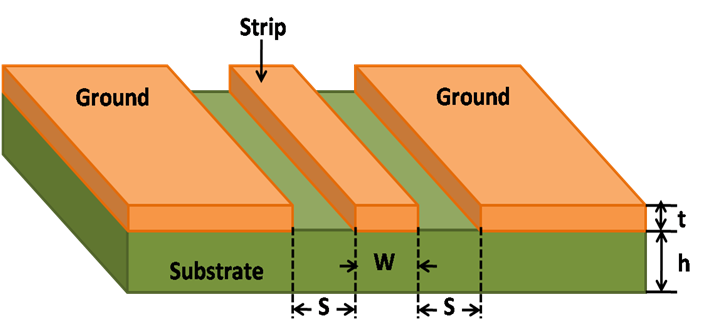
\includegraphics[width=\textwidth]{Figures/DRIE/CPW.png}
        \end{center}
        \caption{Schematic of a coplanar waveguide.}
        \label{fig:CPW}
    \end{wrapfigure}

    In the context of circuit QED, one of the most common types of resonators are coplanar waveguides (CPW). Coplanar waveguides consist of a long central conducting track, with on both sides a neighbouring grounded track. The conducting track is seperated from the grounded tracks by a fixed distance.

    One end is usually capacitively coupled to a feedline and has an open end, while the other end can either be open or shorted. This determines whether the current has a node or an antinode at that end. In the case of a shorted end, current has an antinode at that end, resulting in a quarter wave resonator. This means that the wavelength of the fundamental mode fits a quarter times into the resonator. In the case of an open end, the current has a node at that end, resulting in a half wave resonator.


  \section{Quality factor}
    \label{sec:Quality factor}
    % TODO
    % Find where it says that loss tangents can be added to each other
    % Include the fact that participation ratios are needed for adding quality factors of loss channels
    % Explain why one wants a quality factor that is as high as possible
    The quality of a resonator can be quantified through its quality factor. Generally speaking, the quality factor of a resonator determines the ratio between energy stored in a resonator and the energy leaking away from the resonator. For cQED resonators this corresponds to the rate at which photons dissipate from the resonator. A high quality factor corresponds to a low dissipation rate.

    The quality factor can also be defined in two different ways \cite[pp.23-24]{Mazin}:

    \begin{equation}
        Q = \omega_0 \tau_1 = \omega_0 / \Delta \omega
        \label{eqn:quality factor definition}
    \end{equation}
    Here $\omega_0$ is the resonance frequency of the resonator, and $\tau_1$ is the decay time of the resonator. The decay time is the time taken by a resonator to dissipate its energy to $1/e$ of its original energy.

    Photons can dissipate from the resonator through the resonator's different loss channels. Each of these loss channels has a corresponding quality factor. One such loss channel is due to resonators in cQED being capacitively coupled to a feedline. The quality factor associated to this loss channel is known as the coupling quality factor $Q_c$. This coupling quality factor depends on the amount of capacitive coupling between the resonator and the feedline. It can therefore be engineered to have a certain value, depending on the amount of interaction wanted between resonator and feedline.

    The other loss channels are usually unwanted, and therefore desired to be as low as possible. These individual channels are usually lumped together, resulting in a combined quality factor, known as the intrinsic quality factor $Q_i$.

    The total quality factor of the resonator is known as the loaded quality factor $Q_l$. It is related to $Q_c$ and $Q_i$ through:

    \begin{equation}
        \frac{1}{Q_l} = \frac{1}{Q_c} + \frac{1}{Q_i}
        \label{eq:Q_l}
    \end{equation}

    From equation \ref{eq:Q_l} it can be seen that if the difference between $Q_c$ and $Q_i$ is large, then the loaded quality factor $Q_l$ will be approximately equal to the minimum of the two.


    For a quarter wave resonator the amplitude of transmission has a minimum $S_{21}^{min}$, given by \cite[p29]{Mazin}:
    \begin{equation}
        S_{21}^{min} = \frac{Q_c}{Q_c + Q_i}
        \label{eq:S21min}
    \end{equation}

    With knowledge of the resonant frequency $\omega_0$, the resonant width $\Delta \omega$, and the transmitted signal at resonance $S_{21}^{min}$, it is possible through equations \ref{eqn:quality factor definition} and \ref{eq:S21min} to determine both the coupling quality factor $Q_c$ and the intrinsic quality factor $Q_i$. Note that as equation~\ref{eq:S21min} depends on the ratio of the two quality factors,to get an accurate estimate of both quality factors, they should have a comparable value.

    One reason why a high quality factor is important in the context of cQED is that a qubit can be coupled to a resonator. This qubit therefore experiences dissipation due to its coupling to the resonator, known as the Purcell effect. The result of dissipation is that when the qubit is in its excited state, it will relax to its ground state. The amount of relaxation due to the Purcell effect can be quantified through its relaxation time $T_1^\text{Purcell}$. The reason a high quality factor is important is because the Purcell relaxation time is proportional to the quality factor \cite[p~22]{Geerlings}. The Purcell relaxation time $T_1^\text{Purcell}$ places an upper limit on the relaxation time $T_1$ of a qubit. If the qubit's relaxation time $T_1$ is close to this value, the qubit is said to be Purcell limited.



  \section{Losses}
    \label{sec:Losses}

      When a resonator is being driven at its resonance frequency, it is absorbing photons from the external source. When this external driving stops, the resonator slowly loses its photons through its different loss channels.

      One loss channel has already been discussed in section~\ref{sec:Quality factor}, namely through the coupling to the feedline. This loss channel is not unwanted, as the amount of coupling to the feedline determines how fast the resonator and feedline can interact with each other. The other loss channels, however, are unwanted. They cause dissipation of energy, and hence information. Some of the main causes of loss will be discussed in this section.


  \subsection{Causes of loss}

    \subsubsection{Two-level systems}
      \label{sec:TLS}

      Two-level systems (TLS) are systems which can be in a ground state or in an excited state. In some cases they can be useful. In fact a qubit itself is an example of a TLS. In other cases, however, TLS can also be a source of dissipation such as in the case of dielectric loss \cite{martinis2014ucsb}. Study suggests that in cQED, most TLS reside in a thin oxide layer at the metal-substrate interface and the substrate-air interface \cite{wenner2011surface}.

      Resonators are surrounded by a large quantity of TLS, each of which has its own resonance frequency, depending on its energy landscape. When the resonance frequency of a TLS is close to that of the resonator, it can absorb a photon from the resonator, upon which it tunnels to an excited meta-stable state. TLS have a finite lifetime in their excited state, after which they decay back to their ground state and are then again able to absorb a photon. The rate at which a TLS absorbs a photon depends on the electric field surrounding the TLS.

      In the low power, low temperature regime, TLS reside mostly in their ground state, and only occasionally tunnel to the excited state, upon absorption of a photon. It is theorized that, in this regime, TLS are the main source of dissipation for resonators \cite{gao2008experimental}. At higher powers and/or temperatures, TLS will tunnel to an excited state at a higher rate. Due to their finite lifetime they become saturated at a certain point. Since the quality factor depends on the ratio between energy stored and energy dissipated, when the TLS are saturated the amount of dissipation is limited, while the energy stored in the resonator can still increase. Therefore, in the low power, low temperature regime, increasing either of the two parameters results in an increase in quality factor. At a certain point, however, further increasing either of the two will not improve the quality factor. This is due to other effects dominating the dissipation rate in these regimes.

      % \begin{itemize}
      %     \item 1/f noise \cite{burnett2013evidence}
      %     \item Dielectric materials (Table \cite{martinis2014ucsb})
      % \end{itemize}



    \subsubsection{Quasiparticles}

      Another source of dissipation for resonators is due to quasiparticles being present in the superconducting layer. When a Cooper-pair is broken up, Bogoliubov quasiparticles are formed \cite[p16]{Barends}. Once formed, the quasiparticles have a finite lifetime, depending on the temperature of the system. These quasiparticles can have either electron-like or hole-like properties. They are a source of dissipation for resonators, since they are non-superconducting and therefore cause the surface impedance to be slightly resistive \cite[p18]{Mazin}.

      The breaking up of Cooper-pairs is due to excitations. These excitations can either be thermal, or due to photon absorption. Therefore an increase in temperature or an increase in photon density will result in a higher density of quasiparticles. The quasiparticle density increases exponentially with increasing temperature \cite[p44]{Mazin}.

      % \begin{itemize}
      %     \item Quasiparticle excitation energy $E = \xi^2 + \Delta ^2$,
      %         where $\xi$ is the energy of the single particle in the normal state relative to the Fermi energy \cite{Barends}
      %     \item Increases with increasing frequency
      %     \item Quasiparticles are created through thermal excitation, but can also be excited by photons with $h \nu > 2 \Delta$\cite{Gao}
      %     \item Quasiparticles change the surface impedance of resonators, which can be measured.
      %         This technique is used to create MKID detectors \cite{Gao}
      %     \item "[Surface impedance] change is caused by quasiparticles blocking
      %         the Cooper pairs from occupying some of the electron states (through the exclusion principle), which
      %         modifies the effective pairing energy and reduces the density of pairs."\cite[p3]{Mazin}
      %     \item A lot of information in thesis by Lutchyn \cite{Lutchyn}
      % \end{itemize}




    \subsubsection{Radiation}

      A third source of dissipation is due to radiation from the resonator. This radiation is due to the spontaneous emission of photons.

      The amount of dissipation due to radition is directly related to the geometry of the resonator through \cite{sage2011study,Mazin}:

      \begin{equation}
          Q_\text{rad} = \alpha \left( \frac{L}{s + w}\right)^{n_r}
          \label{Qrad}
      \end{equation}

      As shown in Figure~\ref{fig:CPW}, $s$ is the distance between the conducting and grounded track, $w$ is the width of the conducting track, and $L$ is the length of the resonator. The parameter $\alpha$ depends on properties such as impedance and the dielectric constant of the substrate, and $n_r$ depends on the shape of the resonator, and is equal to 2 in the case of a straight resonator. From Formula \ref{Qrad} it is clear that a decrease of the conducting track width or the distance between tracks leads to an increase in $Q_\text{rad}$. However, with a decrease of either of the two parameters, the field strength close to the resonator becomes higher. If the TLS are not saturated (i.e. low power and temperature), this will increase the amount of dissipation through TLS. Therefore it is not necessarily advantageous to minimize $s$ and $w$.

      Radiation loss becomes the dominant source of dissipation at high powers and/or temperatures, but otherwise usually is not the limiting factor. Since measurements relevant for quantum computing are usually operated at low power and temperature, this source of dissipation is usually less important than other sources, such as TLS dissipation.



    \subsubsection{Vortices}

      When a sample is cooled down to a superconducting state there may still be a small, but nonnegligible magnetic field present. The presence of a magnetic field can cause vortices to appear in superconducting materials. These vortices have a non-superconducting core. Current passing through superconductive materical exerts a Lorentz force on vortices. For a resonator being driven on resonance, this AC current results in the vortices near the resonator experiencing a dissipative oscillatory motion \cite{plourde2009microwave}.

      It is interesting to note that the presence of vortices does not necessarily lead to a lower internal quality factor. The influence of a vortex on a resonator depends on its location. As reported by Nsanzineza et al.~\cite{nsanzineza2014trapping}, a vortex close to a current antinode of a resonator, can result in a significant loss of the quality factor. A vortex close to a current node, however, may even increase the quality factor of the resonator. They attribute this increase in quality factor to quasiparticles, which would otherwise lead to dissipation, being trapped in the vortex.


      % \begin{itemize}
      %     \item Abrikosov vortices
      %     \item worse for thin films?
      %     \item how does movement affect loss?
      % \end{itemize}



  \subsection{Minimizing losses}

  \subsubsection{Surface treatment}

  Previous research has determined that for resonators, TLS are mostly present at the surfaces \cite{gao2008experimental}. These oxides may reside at the interface between metal and dielectric, or between the dielectric and vacuum, or possibly between metal and vacuum (depending on the type of metal used). One explanation for TLS being present is the presence of an amorphous oxide layer at the interfaces. These oxides may act as TLS. During deposition of the metal on the dielectric, this oxide layer can become trapped between the two interfaces. For a silicon dielectric, this oxide layer can be removed by shortly treating the sample with hydrophluoric acid. This process is also known as an 'HF dip'.

  Aside from the HF dip, additional surface treatment can be applied. For the resonators measured in this report, before depositing the metal on the substrate, an additional exposure to hexamethyldisilazane (HMDS) was applied. The reason for this additional step is that there is a lattice mismatch between the metal and substrate. The intermediate layer of HMDS can possibly mediate this lattice mismatch. See \cite{DRIE} for more information.


  \subsubsection{Infrared shielding}

  Aside from thermal excitation, quasiparticles are also formed from the absorption of photons. High-frequency photons (UV-range or higher) are usually not a significant contribution, as they are easily absorbed by materials, well before they reach the inner layers of the fridge. Lower-frequency photons, such as in the infrared range, however, can penetrate through the fridge to the sample. These infrared photons can cause the excititation of quasiparticles. By using infrared shielding, such as a coating film inside the fridge, the amount of infrared radiation reaching the sample can be lowered.



  \subsubsection{Deep-reactive ion etching}

  Another technique applied to the resonators studied in this report is deep-reactive ion etching (DRIE), which is a type of Bosch process \cite{DRIE}. In this technique two alternating steps are performed:

  \begin{enumerate}
      \item An etching step in which an $\chem{SF_6}$ plasma is used to etch the substrate layer.
      \item A passivation step in which $\chem{C_4H_8}$ is released. The gas forms a protective layer on the substrate, except for the direction in which the etching plasma is accelerated. The result is that the sidewalls are protected from the etching process
  \end{enumerate}

  Using DRIE, nearly vertical sidewalls can be created for the substrate. The result is that the substate-air interface is removed from the regions between the CPW tracks, which are the regions where the electric field strength is high. As the dissipation due to TLS depends on the electric field strength, it is expected that DRIE will result in a lower TLS dissipation rate at this interface.

  \subsubsection{Magnetic shielding and vortex trapping}

  Vortices are created when a magnetic field is present. One method to lower the amount of vortices is to use proper magnetic shielding around the sample. Furthermore, using nonmagnetic materials also result in lower amounts of vortices being present.

  Even when using these methods to counter the presence of magnetic fields, there may still be a small amount of vortices present in the sample, which may lead to dissipation. To counter their movement a grid-like structure can be added in the superconducting material, effectively pinning the vortices.



\chapter{Experimental set-up}


  \begin{wrapfigure}{r}{0.4\textwidth}
      \begin{center}
          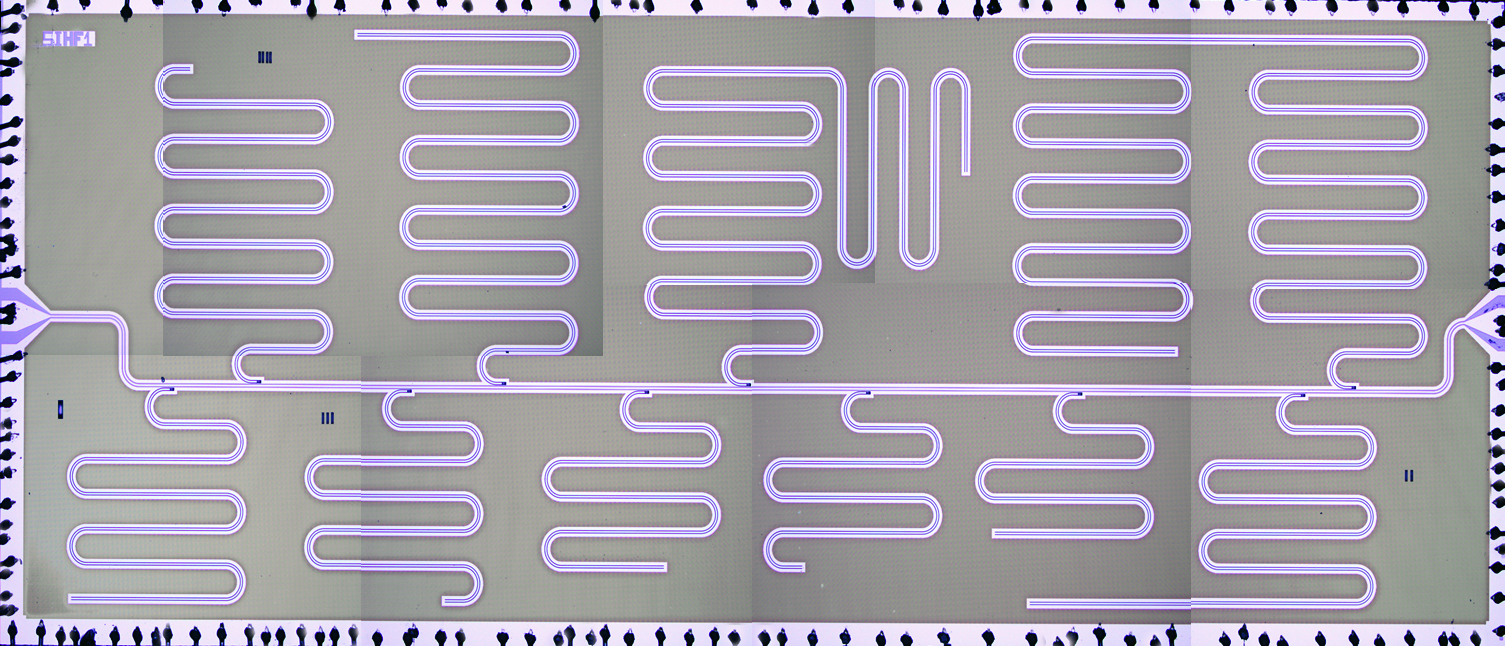
\includegraphics[width=\textwidth]{Figures/DRIE/All_set4.png}
      \end{center}
      \caption{Optical microscopy image of the sample measured in this report. The sample consists of ten quarter wave resonators, with frequencies ranging between \SIrange{1}{11}{\giga \hertz}, connected to a central feedline. The resonators are made using NbTiN on a Si substrate. The sample is treated with HMDS and DRIE.}
      \label{fig:set4}
  \end{wrapfigure}

  The fridge used in this experiment is a dilution refrigerator, made by Leiden Cryogenics. The refrigerator has a base temperature of \SI{\sim15}{\milli \kelvin}. An input signal was generated using a Rohde \& Schwarz ZVM vector network analyzer, connected to an Aeroflex 8310 step attenuator, which has an attenuation range of \SI{120}{\decibel}. The signal out of the fridge was measured using the same vector network analyzer.

  Using this set-up, quarter wave resonators, fabricated by Alessandro Bruno, were measured in a frequency range between \SIrange{1}{9}{\giga \hertz}. The sample is shown in Figure~\ref{fig:set4}. The resonators were made using NbTiN on a silicon substrate. The advantage of NbTiN is that the metal atoms are bound to nitrogen, thereby inhibiting bond formation with oxides. In a way to minimize losses, all resonators were treated with HMDS and deep-reactive ion etching.

  By driving a signal through the feedline, the resulting transmitted signal $S_{21}$ can be measured. At or close to the resonance frequency of a resonator, the resonator will interact strongly with the feed line, resulting in a reduction in transmission.

  Unless stated otherwise, all measurements were performed with the fridge at base temperature (\SI{\sim15}{\milli \kelvin}).

\chapter{Results and discussion}


\section{Resonator measurement}

\begin{figure}[h]
    \centering
    \begin{subfigure}[b]{.49\textwidth}
        \label{fig:resonator_amplitude}
        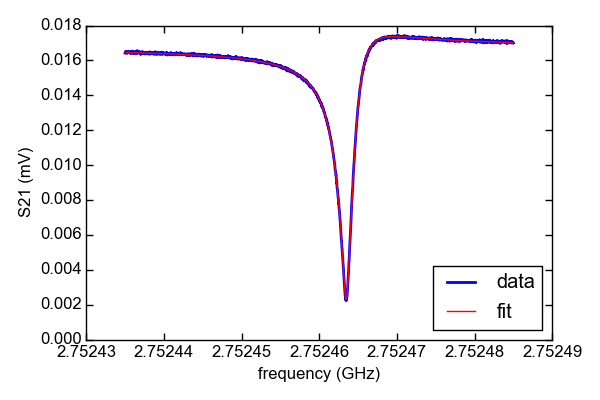
\includegraphics[width=\textwidth]{Figures/DRIE/resonator_amplitude.png}\figureinset{(a)}{2.55}{2.0}
    \end{subfigure}
    \begin{subfigure}[b]{.49\textwidth}
        \label{fig:resonator_complex}
        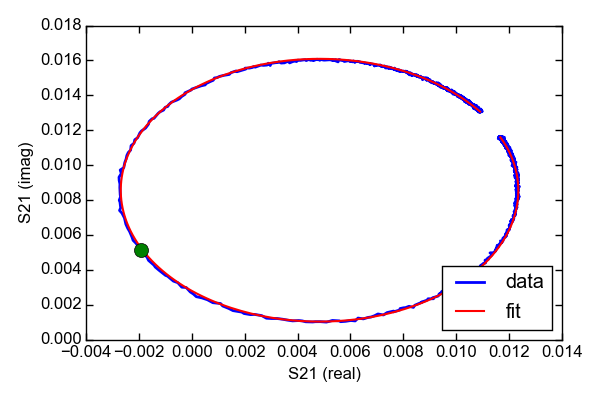
\includegraphics[width=\textwidth]{Figures/DRIE/resonator_complex.png}\figureinset{(b)}{2.55}{2.0}
    \end{subfigure}
    \caption{Forward transmission $S_{21}$ spectrum of a resonator around \SI{2.75}{\giga \hertz}. Panel (a) shows the amplitude of $S_{21}$, along with a fit (red). Panel (b) shows the path of $S_{21}$ in the complex path, along with a fit (red). The green dot indicates the resonance frequency of the resonator.  Measurement was performed at \SI{15}{\milli \kelvin} at an input power of \SI{-123}{\dBm} corresponding to $\sim 5 \times 10^4$ photons.}
    \label{fig:resonator}
\end{figure}

 In Figure~\ref{fig:resonator} the transmission $S_{21}$ of a resonator is shown. Figure~\ref{fig:resonator}(a) shows the transmitted voltage $|S_{21}|$ of the resonator as a function of frequency. As one can see, the resonator has a shape similar to a Lorentzian dip. One interesting point is that the Lorentzian exhibits an asymmetry, which is often attributed to reflections in the feedline \cite[p192]{Geerlings}. This could be caused by impedance mismatching.

 % TODO
 % Say something about complex data

\section{Power dependence}
\label{sec:resonator:results:power_dependence}

\begin{figure}
    \centering
    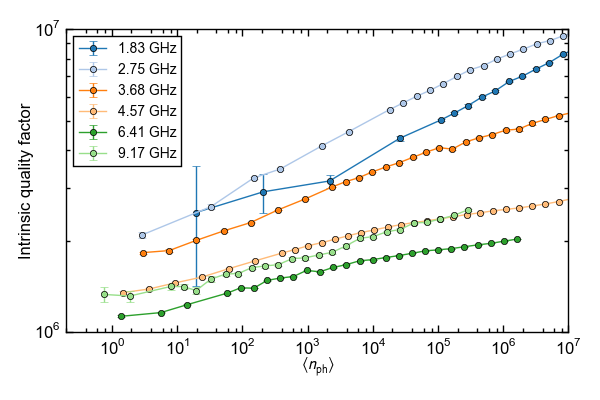
\includegraphics[width=0.8\textwidth]{Figures/DRIE/Qi_vs_n_photon.png}
    \caption{Intrinsic quality factor of resonators as a function of mean number of photons present in the resonator. Measurements were performed at \SI{15}{\milli \kelvin}.}
    \label{fig:Qi_vs_n_photon}
\end{figure}
To be able to study the behaviour of the resonators, measurements were performed for several powers. Using proper calibrations for the attenuation down to the sample, the power can be converted to the input power at the sample. This value can then be converted to the mean number of photons present in the resonator \cite{DRIE}. The results are shown in Figure~\ref{fig:Qi_vs_n_photon}.

As can be seen, the internal quality factor $Q_i$ of all resonators decrease with decreasing photon number. One explanation for this phenomenon is that the dissipation dissipation is mainly due to TLS. Since measurements were performed at \SI{\sim15}{mK}, the TLS are not saturated since the rate of thermal excitation is low. As discussed in section~\ref{sec:TLS}, the relative loss due to TLS is highest at low power, in the regime where they are not saturated. Therefore the fact that the internal quality factor $Q_i$ rises with the mean number of photons present in the resonator can be attributed to a larger amount of TLS being satured. This would suggest that, even with HMDS and DRIE treatment of the sample, at low power and temperature, the internal quality factor is still limited by TLS being present.

The mean photon number of a resonator is inversely proportional to the square of frequency \cite{DRIE}, so for resonators with a low frequency a lower input power is required than with a high frequency. At high photon numbers this is not a concern, as the transmitted signal is high enough to be accurately measured in a short period of time. For the single-photon powers, however, which is the region of interest for quantum computation, acquiring enough signal took up to five hours for the lowest frequencies. The reason that for the resonator with a resonance frequency at \SI{1.83}{\giga \hertz} has large error bars at low powers can be partly attributed to this, but as we will see in section \ref{sec:noise_results}, the main reason is that its frequency lies outside the bandwidth of the amplifiers and circulators of the set-up, resulting in a large amount of additional noise.

% \begin{itemize}
%     \item Quality factor depends on frequency?
%     \item One can also see that the quality factor is lower for resonators with higher resonance frequency.
% \end{itemize}




\section{Temperature dependence}
\label{sec:resonator:results:emperature_dependence}
\begin{figure}
    \centering
    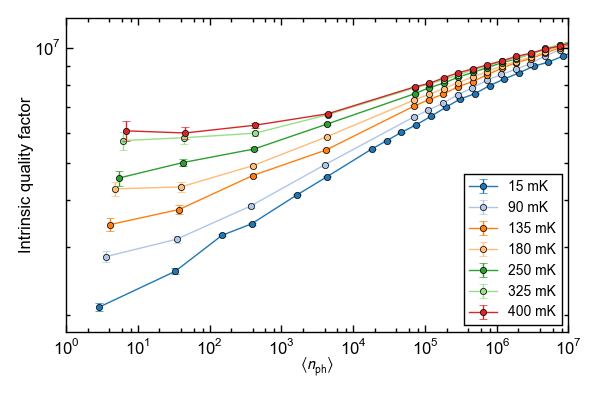
\includegraphics[width=0.8\textwidth]{Figures/DRIE/Qi_vs_n_photon_temperature_dependence.png}
    \caption{Intrinsic quality factor versus photon number for temperatures ranging from \SI{15}{\milli \kelvin} up to \SI{400}{\milli \kelvin}. All measurements were performed for a resonator with resonance frequency $f_0 = $\SI{2.75}{\giga \hertz}.}
    \label{fig:Qi_vs_n_photon_temperature_dependence}
\end{figure}

Aside from power, some of the dissipation channels also depend on the temperature of the system. To be able to study the effect of temperature on resonators, the resonator with frequency \SI{2.75}{\giga \hertz} has been studied as a function of power for several temperatures ranging from \SI{15}{\milli \kelvin} up to \SI{400}{\milli \kelvin}. The reason for choosing this resonator is that it has the highest internal quality factor of all the resonators measured, and so any change in quality factor would be most clearly visible.

The results are shown in Figure~\ref{fig:Qi_vs_n_photon_temperature_dependence}. As can be clearly seen, the quality factor increases with increasing temperature. This is likely due to the fact that TLS are thermally excited for a larger percentage of time. Therefore, the relative energy dissipation with respect to total energy in the resonator will be lower, resulting in an increase in quality factor.

Another interesting point is that the increase in quality factor as a function of temperature is largest at low powers. This can also be explained when the limiting factor is due to TLS. With low powers, the TLS are almost exclusively excited thermally, while at higher powers, the excitation of TLS is not only due to thermal excitations, but also from photon absorption.

If one looks at the highest temperatures, it seems that the increase in quality factor as a function of temperature seems to slowly approach a saturation point. One reason is that the TLS are approaching their saturation, and so increasing the temperature further will have little effect on the percentage of time that the TLS are in the excited state. As will be shown in the next section, at \SI{400}{\milli \kelvin} the quality factor of the resonator is close to its maximum value, and will decrease as temperature is further increased.



\section{Temperature tracking}
\label{resonator:results:temperature_tracking}
\begin{figure}[h]
    \centering
    \begin{subfigure}[b]{.49\textwidth}
        \label{fig:temperature_tracking_Qi_drop}
        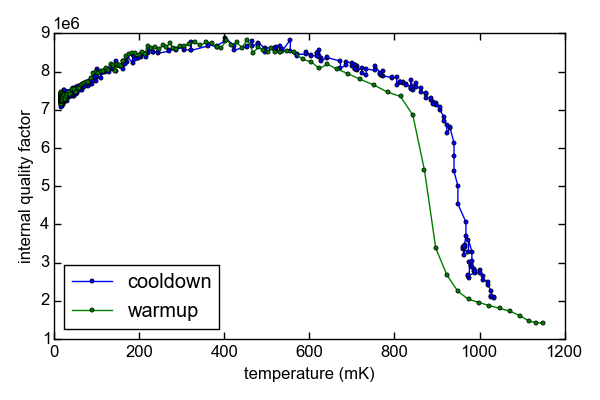
\includegraphics[width=\textwidth]{Figures/DRIE/Temperature tracking drop - Qi vs T.png}\figureinset{(a)}{2.65}{1.92}
    \end{subfigure}
    \begin{subfigure}[b]{.49\textwidth}
        \label{fig:temperature_tracking_Qi_nodrop}
        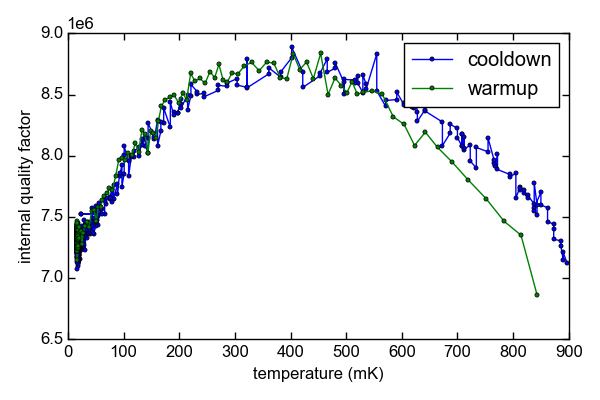
\includegraphics[width=\textwidth]{Figures/DRIE/Temperature tracking - no drop - Qi vs T.png}\figureinset{(b)}{2.57}{1.92}
    \end{subfigure}
    \caption{Internal quality factor versus temperature for the resonator with resonance frequency $f_0= $\SI{2.75}{\giga \hertz}. Quality factor was continuously measured as the sample was cooled down and warmed up four days later. Panel (a) shows the full temperature range up to the helium condensation cycle. Panel (b) shows a close-up of the region until \SI{900}{\milli \kelvin}.}
    \label{fig:temperature_tracking_Qi}
\end{figure}

To further investigate the temperature dependence of the resonator, a continous measurement was performed on the resonator with resonance frequency \SI{2.75}{\giga \hertz} during a cool-down and a subsequent warm-up of the fridge four days later. Measurements were performed for temperatures ranging from base temperature (\SI{15}{\milli \kelvin}) to roughly \SI{1}{\kelvin}. Above this temperature, the fridge entered a cyclic helium condensation/evaporation process. All temperatures were measured at an input power of \SI{-113}{\dBm}, corresponding to roughly $5 \times 10^5$ photons. In Figure \ref{fig:temperature_tracking_Qi} the internal quality factor versus temperature is shown during a cooldown and subsequent warm-up of the fridge. As can be seen, the quality factor reaches a maximum quality factor at a temperature of \SI{\sim400}{\milli \kelvin}. Below this temperature, the quality factor is likely limited by the presence of TLS (see sections \ref{sec:resonator:results:power_dependence} and \ref{sec:resonator:results:emperature_dependence}). Above this temperature however, the quality factor decreases, indicating that TLS are not the limiting factor anymore for $Q_i$. One likely explanation is that the main source of dissipation is now due to the presence of quasiparticles in the resonator. At even higher powers other effects, such as vortices and enhanced radiation, contribute more and more significantly to the decay of the quality factor.

From Figure~\ref{fig:temperature_tracking_Qi} it seems that there is some hysteresis at high temperatures. However, this is likely due to the fact that the thermometer is at a different position in the fridge as the sample, and does not thermalize equally fast. There may therefore be a delay between the temperature of the thermometer, and the actual temperature of the sample.

\begin{figure}[h!]
    \centering
    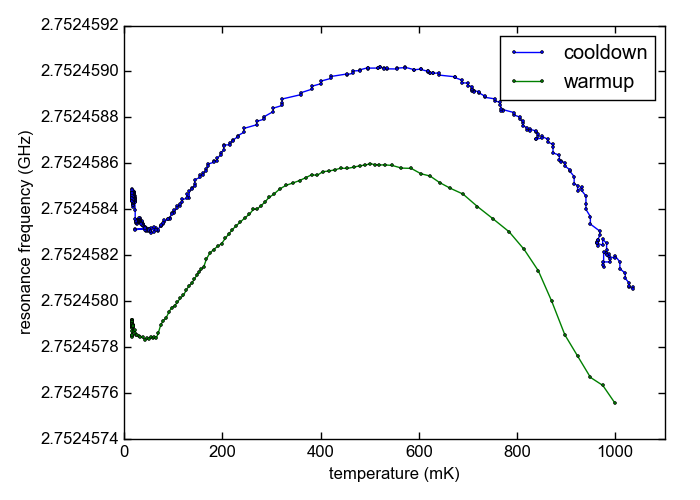
\includegraphics[width=.72\textwidth]{Figures/DRIE/Temperature tracking - f0 vs T.png}
    \caption{Resonance frequency versus temperature during a cooldown and subsequent warm-up four days later. In the period between cooldown and warm-up the resonance frequency has shifted by \SI{\sim 500}{\hertz}, possibly due to phase noise.}
    \label{fig:temperature_tracking_f0}
\end{figure}


Aside from the internal quality factor, another quantity of interest is the resonance frequency $f_0$ of the resonator, which also depends on the temperature. The result from of tracking the resonance frequency of the resonator during cooldown and subsequent warm-up is shown in Figure~\ref{fig:temperature_tracking_f0}. As can be seen in both cases, the resonance frequency reaches a maximum around \SI{500}{\milli \kelvin}.

Between the cooldown and warm-up the resonance frequency seems to have shifted by roughly \SI{500}{Hz}. As the sample was kept at \SI{15}{\milli \kelvin}, it is unlikely that this decrease in resonance frequency is due to degradation of the sample. One possible explanation is that this change in resonance frequency is due to phase noise, which is known to shift the resonance frequency of the resonator. Further measurements are, however, required to determine if this is the case.

The decrease in resonance frequency at higher temperatures can be explained by the presence of quasiparticles, which increase the kinetic inductance \cite[p91]{Geerlings}. The resonance frequency is inversely proportional to the square root of the total conductance \cite{barends2008contribution}, and so an increase in kinetic inductance leads to a decrease in resonance frequency. For measurements done by Barends et al. \cite{barends2008contribution}, the change in resonance frequency due to changes in the kinetic inductance seem to roughly correspond with the decrease in center frequency measured in Figure~\ref{fig:temperature_tracking_f0}.

\begin{figure}[h]
    \centering
    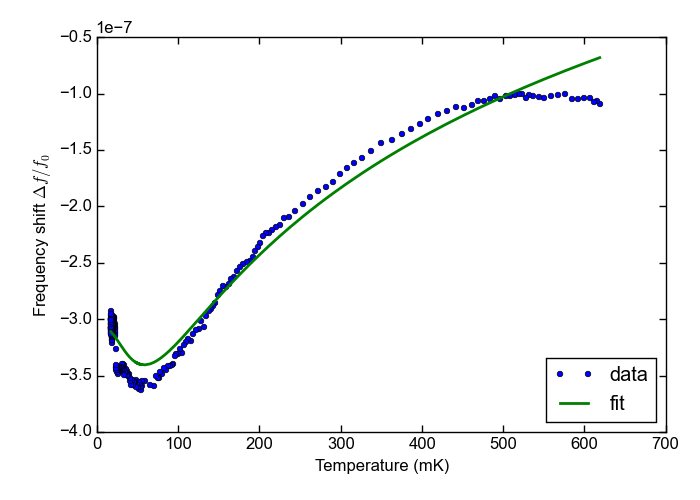
\includegraphics[width=.7\textwidth]{Figures/DRIE/Temperature increase tracking - f0 vs T with fit.png}
    \caption{Frequency shift versus temperature for low temperatures, along with fit (green). The fit was performed using the model by Gao et al.~\cite{gao2008experimental}. The fit corresponds well with data, even describing the frequency peak at the lowest temperatures.}
    \label{fig:f0_vs_T_with_fit}
\end{figure}

The decrease in resonance frequency at lower temperatures can be explained due to TLS still being present. A model is presented by Gao et al. \cite{gao2008experimental}, in which they describe the decrease in resonance frequency due to the presence of TLS. As can be seen in Figure~\ref{fig:f0_vs_T_with_fit} the model corresponds well with the data at low temperatures. At higher temperatures the model deviates from data, which may be explained by quasiparticles dominating as source of dissipation. An interesting thing to note is that an increase in resonance frequency was predicted at the lowest temperatures, but as they did not reach temperatures sufficiently low they could not confirm this effect. In Figure~\ref{fig:f0_vs_T_with_fit} however, this increase in resonance frequency is observed. This supports the claim that at low temperatures the resonator is still limited by TLS, even after treatment of HMDS and DRIE.



\chapter{Conclusion and future work}

Since the quality factor of all resonators is found to decrease with decreasing input power, this indicates that at low temperatures and powers the limiting factor is still due to TLS. The fact that the quality factor initially increases with higher temperatures, supports this claim. By also measuring  the resonance frequency as a function of temperature, the curve obtained is in good agreement with a model describing the resonance frequency shift due to TLS \cite{gao2008experimental}. The curve even shows an increase in resonance frequency at the lowest temperatures, which was also predicted by the model. These results suggest that even after HMDS surface treatment and deep-reactive ion etching was applied, the internal quality factor of the resonator at low temperatures and power is still limited by the presence of TLS.

Nevertheless, As shown by Bruno et al. \cite{DRIE}, the application of HMDS surface treatment and DRIE resulted in an improvement of the internal quality factor of the resonators by almost an order of magnitude. More research must be done to determine at what interface the dissipation due to TLS is greatest after these two treatments.

The next step is to perform the same treatments (HMDS and DRIE) on transmon qubits, to study what the influence will be on coherence times.
